\documentclass[11pt]{article}

% Generated by paper/build/build.py from paper/source/score.md. Do not edit.
\usepackage{iftex}
\ifPDFTeX
  \usepackage[T1]{fontenc}
  \usepackage[utf8]{inputenc}
  \usepackage{lmodern}
  \usepackage{textcomp}
\else
  \usepackage{fontspec}
\fi
\usepackage{amsmath,amssymb}
\usepackage{longtable,booktabs,array,calc}
\usepackage{graphicx}
\usepackage{xcolor}
\usepackage[numbers,sort&compress]{natbib}
\usepackage{microtype}
\usepackage[margin=2.5cm]{geometry}
\usepackage[colorlinks=true,linkcolor=blue,citecolor=blue,urlcolor=blue]{hyperref}
\providecommand{\tightlist}{\setlength{\itemsep}{0pt}\setlength{\parskip}{0pt}}
\providecommand{\pandocbounded}[1]{#1}
\setlength{\emergencystretch}{3em}

\title{SCORE: A Framework for Synthesizing Complete, Owned, Responsive
Environments}
\author{J.P. Kardolus, Babon Innovations B.V., Utrecht, The Netherlands}
\date{Working draft, 8 October 2026}

\begin{document}
\maketitle
\begin{abstract}
World models and one-shot 3D generators produce a convincing place from
a sentence or a picture, but not a world a creator can build on: a
stream of frames, or one fused scene without separate objects,
collision, logic or clear rights. SCORE is a world generation framework
that joins many open vision foundation models, procedural tools and
coding agents into one route from a creator's picks to a complete world
in the creator's own engine. Every object is its own model, every
surface comes from one shared rule-based library, sound is generated for
every surface, room and object, and every model in the route allows
commercial use of its output. The work runs offline in cloud batches
through stages whose outputs are kept, so a weak result can be traced to
the stage that caused it, rerun or fixed there, and regenerated without
losing the creator's edits. Deterministic checks gate every paid step,
and the creator decides the look, the concept and the style and reviews
each place with tools the framework supplies. We describe the framework
and apply it to four worlds of different kinds.
\end{abstract}


\section{Introduction}\label{introduction}

A creator who wants a world for a game, a film or a robot to train in needs it complete and owned. Complete means every door, floor, object, light and sound exists and works when the player looks anywhere. Owned means the creator decides what the world is, can change any part later without starting over, and holds the rights to all of it.

World models make the first impression of a world cheap but give neither. Genie 3 renders a world a person can move through in real time, with a constrained range of actions and a few minutes of continuous interaction among its stated limits \citep{genie3, bruce2024genie}. One-shot 3D world generators return ``static monolithic assets with limited editability and physical interaction'' \citep{hu2026worldact}.

SCORE takes the opposite approach. It builds everything in full, offline, so the world cannot break and can be used today in the engines and tools the creator already has. The creator writes the score; coding agents and open tools play it. The creator decides at a few fixed points (references, concept, style, review). Between them, every stage hands on explicit data or code that an agent can read and a deterministic check can test before money is spent, and the agents do the joining work a technical artist would otherwise do.

Our contributions are: SCORE as a world compiler, with its stages, canonical scene and checks (Section 3); the rules that keep generated worlds coherent and editable, chiefly the parts check, one model per object and a shared surface library (Sections 3.3 and 3.4); and four worlds of different kinds built with it, with time, cost and the faults caught before spending at every stage (Section 5).

\section{Related work}\label{related-work}

\textbf{World models and world generators.} Genie learns an interactive environment from video \citep{bruce2024genie}. WorldGen generates traversable, editable worlds from text \citep{wang2025worldgen}; WorldAct decomposes a monolithic generated world into objects after the fact \citep{hu2026worldact}; WorldSculpt composes per-object meshes from grounded video \citep{niu2026worldsculpt}. SCORE ships no world-model output; a world generator may appear only as an optional reference step (Section 3.6).

\textbf{Agents that build scenes.} Holodeck has a language model write spatial constraints for a solver \citep{yang2024holodeck}; SceneCraft and recursive code world models write scenes as programs and compare renders with a reference \citep{hu2024scenecraft, li2026rcwm}; WorldClaw and AutoUE use agents to assemble open worlds and game code \citep{guo2026worldclaw, yin2026autoue}; 3D-RE-GEN and SceneConductor decompose one picture into placed objects \citep{sautter2025regen, kim2026sceneconductor}. LEGO-Anything is closest in spirit: its coding agents show ``weak scene initialization, regressive edits during iteration, and unreliable self-evaluation'', addressed with tools rather than training \citep{li2026lego}. SCORE shares that position but builds worlds that do not exist yet, to a person's picks.

\textbf{Procedural generation, parts and style.} Infinigen and Infinigen Indoors generate worlds and rooms from rules, with materials as their own generators \citep{raistrick2023infinigen, raistrick2024indoors}; ProcFunc gives these generators an interface on which language models make far fewer coding errors \citep{raistrick2026procfunc}. PartCrafter and Point2Part split shapes into parts \citep{lin2025partcrafter, tsui2026point2part}. Keeping one style across generated assets is named as open \citep{wu2026production, yang2026flowscene}; Hunyuan3D Studio fixes it at the picture \citep{lei2025hunyuanstudio}. SCORE instead takes surface out of the generated models altogether.

\section{Method}\label{method}

\subsection{A world compiler}\label{a-world-compiler}

SCORE compiles a world once, offline, in batches; nothing is generated while it is played, and each scale of a world (a room, a planet's ground, an orbit) is its own kind of world. Table 1 lists the stages. Each stage's output is explicit, cached and checked before the next paid stage starts.

\textbf{Table 1.} Stages, their outputs and the checks that gate the next stage.

{\def\LTcaptype{none} % do not increment counter
\begin{longtable}[]{@{}
  >{\raggedright\arraybackslash}p{(\linewidth - 4\tabcolsep) * \real{0.3333}}
  >{\raggedright\arraybackslash}p{(\linewidth - 4\tabcolsep) * \real{0.3333}}
  >{\raggedright\arraybackslash}p{(\linewidth - 4\tabcolsep) * \real{0.3333}}@{}}
\toprule\noalign{}
\begin{minipage}[b]{\linewidth}\raggedright
Stage
\end{minipage} & \begin{minipage}[b]{\linewidth}\raggedright
Output
\end{minipage} & \begin{minipage}[b]{\linewidth}\raggedright
Check before the next stage
\end{minipage} \\
\midrule\noalign{}
\endhead
\bottomrule\noalign{}
\endlastfoot
Concept & picked concept picture & creator's pick \\
Plan & dimensioned plan in metres & room and door checks \\
Inventory & every object as a row; children on parents & concept-density check \\
Close-ups & one clean picture per object & one object per picture \\
Shape & code builder or picture-to-3D model per kind & parts check, model check \\
Surfaces & baked maps from the shared library & palette sweep, storage budget \\
Sound & sound per surface, room and object & loudness and fault checks \\
Assembly & the OpenUSD scene and engine builds & scene check, made-only check \\
Review & shots from fixed cameras & creator's keep or send-back \\
\end{longtable}
}

\textbf{The canonical scene.} All stages write one OpenUSD stage \citep{openusd} with glTF geometry \citep{gltf2}. Every object carries its name, kind, place in metres, collision, the library surface of each part, its sound, and tags for what a person can do with it (door, seat, terminal, airlock). The compiler owns a generated base layer and may rewrite it; the creator's changes live in edit layers above it, so a regeneration replaces the base and keeps the edits. Engines and simulators (Godot, Blender, Unreal, robotics simulators) load the same stage through thin adapters.

\subsection{Checks before spending}\label{checks-before-spending}

A fault costs nothing in the plan, cents at the picture, about €0.18 and 75 minutes at the 3D model, and an evening of the creator's time once a room is built and played. Each paid stage is therefore gated by deterministic checks on real geometry, never by an agent's judgement, and a failure sends work back one stage. Room checks cast rays for leaks through walls and roof, pieces blocking openings and pieces off their surface, in about two seconds a room. A door check requires every door to separate its two sides. A concept-density check requires every element of the concept to have an inventory row or a written reason. A model check requires closed solids with walls of at least 3 mm and fails generated boxes that lean more than 2 degrees. A palette sweep and a storage budget per room follow, and after assembly a scene check finds what floats or sinks and fails on any visible mesh the route did not make.

\subsection{Code or pipeline, one model per object}\label{code-or-pipeline-one-model-per-object}

Picture-to-3D models build chunky solids well and flat panels, thin beams and openings badly; agent-written code builders are exact, light and straight, but show only the parts the agent wrote. SCORE routes each object kind by the \textbf{parts check}: a kind is built in code only when its code build shows every part its clean close-up shows, each at least 10 percent visible and none under a label. Every other kind goes through the prop pipeline: Pixal3D \citep{li2026pixal3d} in a cloud batch, closed into a solid, triangles set by size. Composites are split before generation, one model per real-world object: a tool board is a board carrying its tools, a console its monitors and keyboards, each made on its own.

\subsection{Surfaces and sound}\label{surfaces-and-sound}

Models and code give shape only. Every part takes one surface from a shared library of ProcFunc functions \citep{raistrick2026procfunc} on Infinigen's shaders \citep{raistrick2023infinigen}, coloured from the place's palette, with wear, dirt and seed as named settings. A room has one wear setting, applied from causes: edges, foot traffic, drips. Parts of a generated model come from PartCrafter \citep{lin2025partcrafter}, and each part takes one surface, chosen from its picture. Labels are a few decals on clear flat spots. Sound is compiled the same way: each surface carries its footsteps and impacts, each room its echo from its size and surfaces, each object its own sound, generated in one batch by MOSS-SoundEffect \citep{moss2026}, chosen by CLAP prompt match \citep{wu2022clap} less measured faults, and levelled under a -3 dBTP true peak. The libraries of surfaces and sounds grow with each world and are reused in the next.

\subsection{Cloud batches and human picks}\label{cloud-batches-and-human-picks}

Every heavy step runs in a rented cloud machine that is deleted afterwards, records its cost per batch, and stops itself when its output grows past its expected size. The creator picks at fixed points only. Where two routes compete the pick is blind: both drawn the same way, labelled X and Y at random.

\subsection{The optional world step}\label{the-optional-world-step}

A concept shows one view. An optional world step turns it into a walkable whole-room reference, so close-ups can show every object from every side and the walls the concept does not show can be filled in its style. World Labs Marble served this step in our runs; its output is never shipped, and anything derived from it is credited ``Generated using World Labs''.

\section{Implementation}\label{implementation}

SCORE runs as Python tools for planning, routing, baking, assembly and checks, with headless Blender \citep{blender} and rented NVIDIA L4 machines for every heavy step. Claude Code agents \citep{claudecode} write the plans, inventories and code builders under one creator's direction. Table 2 lists the models; each allows commercial use of its output.

\textbf{Table 2.} Models in the route.

{\def\LTcaptype{none} % do not increment counter
\begin{longtable}[]{@{}
  >{\raggedright\arraybackslash}p{(\linewidth - 4\tabcolsep) * \real{0.3333}}
  >{\raggedright\arraybackslash}p{(\linewidth - 4\tabcolsep) * \real{0.3333}}
  >{\raggedright\arraybackslash}p{(\linewidth - 4\tabcolsep) * \real{0.3333}}@{}}
\toprule\noalign{}
\begin{minipage}[b]{\linewidth}\raggedright
Model
\end{minipage} & \begin{minipage}[b]{\linewidth}\raggedright
Role
\end{minipage} & \begin{minipage}[b]{\linewidth}\raggedright
Licence
\end{minipage} \\
\midrule\noalign{}
\endhead
\bottomrule\noalign{}
\endlastfoot
Nano Banana Pro \citep{nanobananapro} & concepts, close-ups & paid API \\
Pixal3D \citep{li2026pixal3d} & picture to 3D & MIT; DINOv3 licence for its encoder \\
PartCrafter \citep{lin2025partcrafter} & parts & MIT \\
Depth Anything V2 Small \citep{yang2024dav2} & ground relief & Apache-2.0 \\
ProcFunc, Infinigen shaders & surfaces & BSD-3-Clause \\
MOSS-SoundEffect, CLAP & sound & Apache-2.0 \\
World Labs Marble \citep{marble_terms} & optional world step & paid; outputs owned by paid users \\
\end{longtable}
}

\textbf{Lessons from development.} The rules above came out of six rounds on one room, the central hub of the game 2099, each answering the creator's verdict on the last. Three findings shaped the method. Deterministic checks catch what agents miss: the first round's room checks cut light leaking through walls and roof from 1.53 percent of 5,817 rays to zero, but only walking the loaded room showed 26 old models still in it, which became the made-only check. Keeping each picture's own colours made every piece bring its own wear, so the creator judged the room messy; surfaces now come only from the library. And generated composites melted their parts together and generated boxes leaned (one locker by 13 degrees), which led to one model per object and the straightness check. The creator preferred the new route in both blind comparisons and accepted the sixth round.

\section{Case study: the world of 2099}\label{case-study-the-world-of-2099}

2099 is a first-person automation game on a Moon base, with a prologue on Earth and a Mars expedition camp. Its central room, the hub, served as the test bench for the route; the rest of the world was then built on the route the hub settled.

\subsection{The hub in six rounds}\label{the-hub-in-six-rounds}

The hub's structure came from a cutaway the creator picked from twenty drawn from his reference pictures (Figure 1). It was then rebuilt six times on 6 and 7 October 2026 (Table 2).

\begin{figure}
\centering
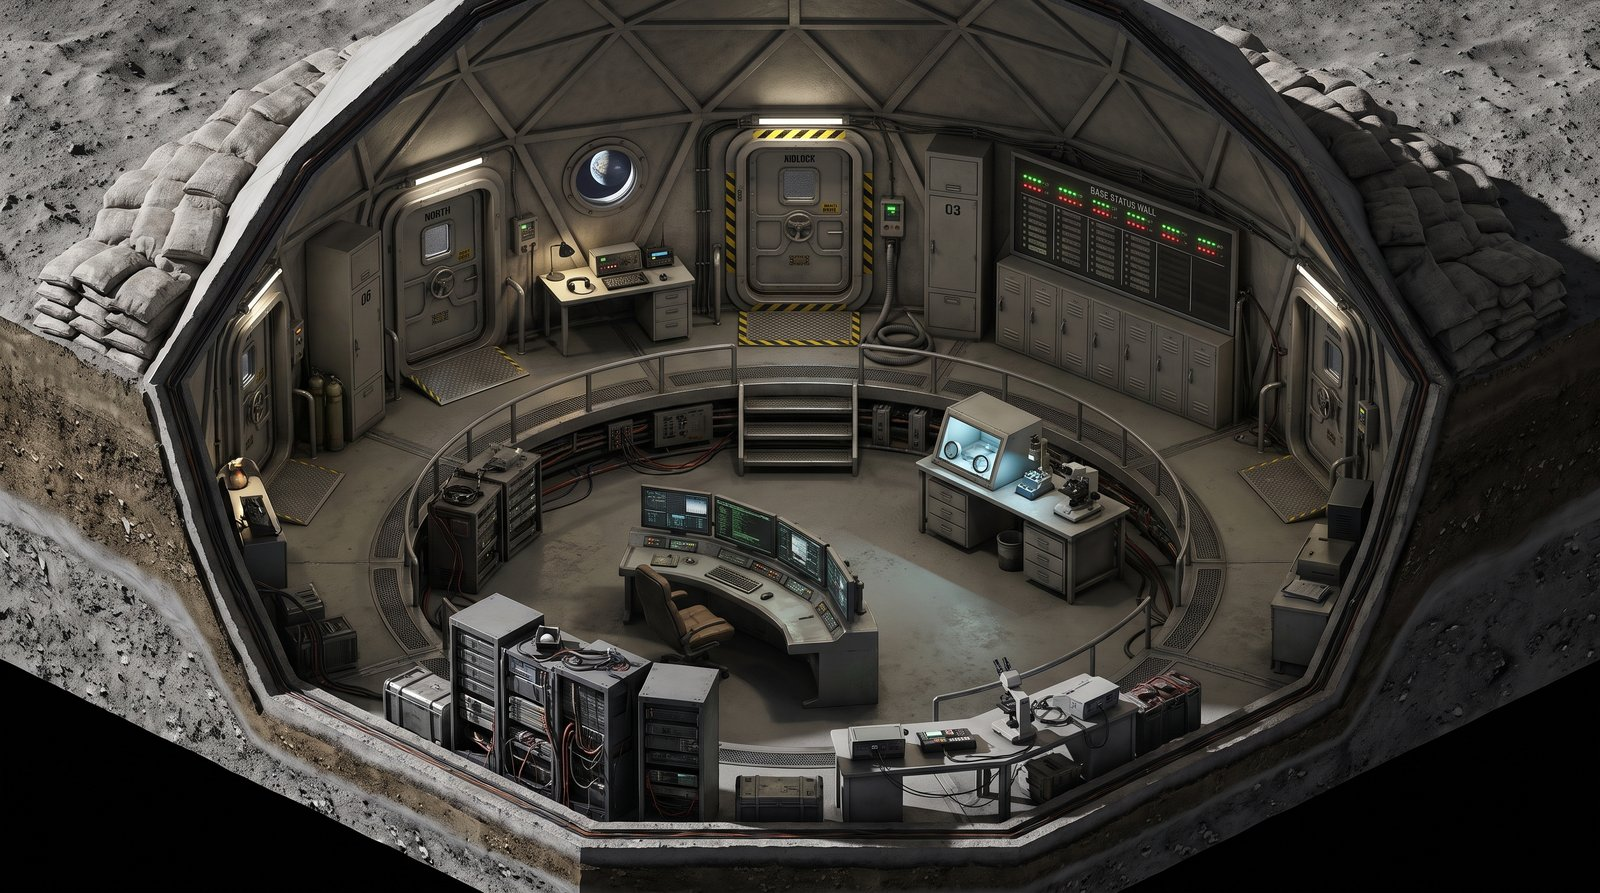
\includegraphics[width=0.8\linewidth,height=\textheight,keepaspectratio,alt={The picked concept for the hub (cutaway C12): a twelve-sided shell over a sunken pit, drawn by Nano Banana Pro from reference pictures the creator kept. It fixes the room's structure and is not shipped.}]{figures/hub-concept-c12.jpg}
\caption{The picked concept for the hub (cutaway C12): a twelve-sided shell over a sunken pit, drawn by Nano Banana Pro from reference pictures the creator kept. It fixes the room's structure and is not shipped.}
\end{figure}

\textbf{Table 2.} The hub's six rounds. Cost is rented GPU time (€) and picture calls (\$). Frame time is the mean on an RTX 5080 at night, 1600×900.

{\def\LTcaptype{none} % do not increment counter
\begin{longtable}[]{@{}
  >{\raggedright\arraybackslash}p{(\linewidth - 8\tabcolsep) * \real{0.2000}}
  >{\raggedright\arraybackslash}p{(\linewidth - 8\tabcolsep) * \real{0.2000}}
  >{\raggedright\arraybackslash}p{(\linewidth - 8\tabcolsep) * \real{0.2000}}
  >{\raggedright\arraybackslash}p{(\linewidth - 8\tabcolsep) * \real{0.2000}}
  >{\raggedright\arraybackslash}p{(\linewidth - 8\tabcolsep) * \real{0.2000}}@{}}
\toprule\noalign{}
\begin{minipage}[b]{\linewidth}\raggedright
Round
\end{minipage} & \begin{minipage}[b]{\linewidth}\raggedright
Change
\end{minipage} & \begin{minipage}[b]{\linewidth}\raggedright
Creator's verdict
\end{minipage} & \begin{minipage}[b]{\linewidth}\raggedright
Cost
\end{minipage} & \begin{minipage}[b]{\linewidth}\raggedright
Frame time
\end{minipage} \\
\midrule\noalign{}
\endhead
\bottomrule\noalign{}
\endlastfoot
1, two walls, A/B & surface library, routing by shape, room checks & blind pick for the new route (``Y looks much cleaner'') & €0.88 & 7.81 ms vs 7.53 \\
2, two walls, A/B & 71-variant library, shared texture sets, roof check & blind pick for the new route & €1.70 & 8.05 ms vs 8.24 \\
3, whole room & route end to end, 74 models & old models still loaded; labels and floor fittings wrong & €1.67 & 6.78 ms (old 9.22) \\
4, whole room & detail through the pipeline, picture colours kept & ``pretty much all of this became messy'' & €8.50, \$5.09 & 9.6 ms \\
5, eight pieces, A/B & shape only from the pipeline, library surfaces, parts check & new method preferred for door, notice board, porthole; three pieces still wrong & €0.21 & not run \\
6, whole room & round 5 everywhere, one model per object, straightness check & ``this looks amazing, I have no negative feedback'' & €3.48, \$1.07 & 5.6 ms \\
\end{longtable}
}

Three findings came out of it. First, deterministic checks found what agents missed: in round one, light escaping through walls and roof fell from 1.53 percent of 5,817 rays to zero, and colour noise within surfaces from a median of 31.1 to 3.2 percent. They did not find what only play showed: in round three 26 old models were still loaded, which led to the check that fails on any visible mesh the route did not make. Second, the split between code and pipeline was the hard decision: routing by shape lost detail (round three), keeping each picture's colours made every piece bring its own wear (round four), and the parts check with library-only surfaces and one model per object was what the creator accepted (Figure 2). Third, consistency and cost moved together: round six drew 0.45 million triangles against round four's 1.96 million, at 5.6 against 9.6 ms a frame and 187 against 487 MB on disk.

\begin{figure}
\centering
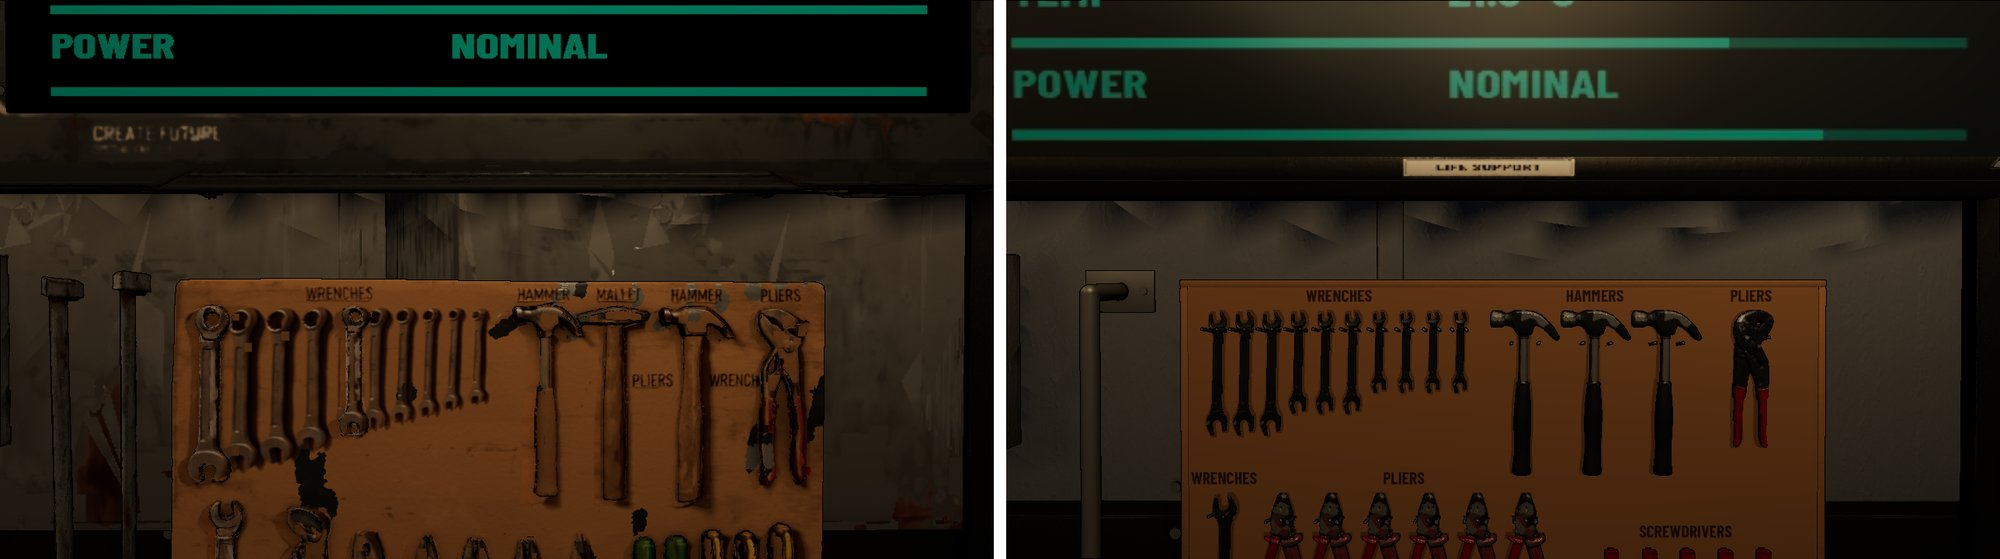
\includegraphics[width=1\linewidth,height=\textheight,keepaspectratio,alt={The hub's tool board in round four (left: one generated model with its picture's colours over library surfaces) and round six (right: a code-built board with 26 separately made tools, library surfaces only). Same camera and build.}]{figures/hub-toolboard-r4-r6.jpg}
\caption{The hub's tool board in round four (left: one generated model with its picture's colours over library surfaces) and round six (right: a code-built board with 26 separately made tools, library surfaces only). Same camera and build.}
\end{figure}

\subsection{The rest of the world}\label{the-rest-of-the-world}

After the hub was accepted, the route was run on the other places in parallel, about one agent per place, from the evening of 7 October until the game work was paused at noon on 8 October. The per-place records (21 entries) cover the planned Moon ground, the old station and the wreck, the base's lab, workshop, greenhouse, habitat, airlock and walkway tubes, the prologue's flat, stairwell, street, square and launch view, and the Mars ground, camp grounds and habitat. Together they record €46.67 of rented GPU time and \$40.72 of picture calls, as floors from the agents' notes, and 971 models: 865 code builders and 106 through the prop pipeline. Single places mostly cost a few euros, while their wall time ran to many hours, much of it waiting for machines and quotas.

The creator accepted the old station and the wreck on first sight (``it just looks great''), and preferred the planned Moon ground to a crater generated with Infinigen, in a comparison that was not blind because the two were rendered differently. The other places are built and pass their checks, but have not been reviewed by the creator in play: the game work was paused before that review, so their acceptance is open. The weaknesses were consistent across places. Code builders gave clean pieces but sparse rooms, and do not scale: each kind needs an agent to write a builder. Rooms read sparser than their concepts, which a concept shows from one side only; this gave rise to the concept-density check. Choosing surfaces by picture colour produced patchy materials. And the pace was set by daily picture quotas and GPU stock, not by compute cost. A count of faults caught per check, before and after spending, belongs here and is not given: the per-place records hold the faults as free text, which still has to be coded by hand.

\section{Evaluation}\label{evaluation}

\begin{center}\fbox{\begin{minipage}{0.94\linewidth}\setlength{\parskip}{4pt}\small

\textbf{Gap: LEGO-Bench.} This section will report SCORE's scores on LEGO-Bench \citep{li2026lego}, a benchmark of scenes rebuilt from pictures. It waits until the benchmark's code is released and until SCORE's scene export and its Blender adapter are built.

\end{minipage}}\end{center}

\subsection{With and without the agent tools}\label{with-and-without-the-agent-tools}

The tools that check an agent's work (the completion gate, the resting triage with its drop test, the pick lock and the render-and-compare, Section 2) were tested on three places of world 1: a room (the workshop, 814 objects), an outdoor place (the street, 1,198 objects) and a dense room (the hangar, 1,657 objects). Each arm started from the same exported stage and the same inventory, and the same agent (Claude Opus 5.5 in Claude Code, headless) got the same prompt: make the place as complete as it can in about 50 minutes, through the place's layout data only. One arm had the framework as it was before these tools; the other had them. Both arms were measured afterwards with the same instruments (Table 2). Each arm ran once, so the table shows what happened, not an average.

\textbf{Table 2.} One session per arm and place. Faults are the resting triage's real faults left on the final stage, measured against the arm's own data; placeholders by the placeholder check; rows are inventory rows with no object and no written reason. Agent cost is the session's model cost in dollars; cloud is what its rented machines cost.

{\def\LTcaptype{none} % do not increment counter
\begin{longtable}[]{@{}
  >{\raggedright\arraybackslash}p{(\linewidth - 18\tabcolsep) * \real{0.1000}}
  >{\raggedright\arraybackslash}p{(\linewidth - 18\tabcolsep) * \real{0.1000}}
  >{\raggedright\arraybackslash}p{(\linewidth - 18\tabcolsep) * \real{0.1000}}
  >{\raggedright\arraybackslash}p{(\linewidth - 18\tabcolsep) * \real{0.1000}}
  >{\raggedright\arraybackslash}p{(\linewidth - 18\tabcolsep) * \real{0.1000}}
  >{\raggedright\arraybackslash}p{(\linewidth - 18\tabcolsep) * \real{0.1000}}
  >{\raggedright\arraybackslash}p{(\linewidth - 18\tabcolsep) * \real{0.1000}}
  >{\raggedright\arraybackslash}p{(\linewidth - 18\tabcolsep) * \real{0.1000}}
  >{\raggedright\arraybackslash}p{(\linewidth - 18\tabcolsep) * \real{0.1000}}
  >{\raggedright\arraybackslash}p{(\linewidth - 18\tabcolsep) * \real{0.1000}}@{}}
\toprule\noalign{}
\begin{minipage}[b]{\linewidth}\raggedright
Place, arm
\end{minipage} & \begin{minipage}[b]{\linewidth}\raggedright
Real faults (start → end)
\end{minipage} & \begin{minipage}[b]{\linewidth}\raggedright
Placeholders
\end{minipage} & \begin{minipage}[b]{\linewidth}\raggedright
Rows missing
\end{minipage} & \begin{minipage}[b]{\linewidth}\raggedright
Minutes
\end{minipage} & \begin{minipage}[b]{\linewidth}\raggedright
Agent cost
\end{minipage} & \begin{minipage}[b]{\linewidth}\raggedright
Output tokens
\end{minipage} & \begin{minipage}[b]{\linewidth}\raggedright
Cloud
\end{minipage} & \begin{minipage}[b]{\linewidth}\raggedright
Exports
\end{minipage} & \begin{minipage}[b]{\linewidth}\raggedright
Gate said unknown
\end{minipage} \\
\midrule\noalign{}
\endhead
\bottomrule\noalign{}
\endlastfoot
Workshop, without & 18 → 13 & 0 → 0 & 1 → 0 & 36 & \$2.26 & 30.4k & €0.85 & 7 & not used \\
Workshop, with & 18 → 0 & 0 → 0 & 1 → 0 & 26 & \$1.42 & 14.3k & €0.85 & 2 & 2 of 4 calls \\
Street, without & 11 → 0 & 0 → 0 & 0 → 0 & 38 & \$2.40 & 30.0k & €0.32 & 9 & not used \\
Street, with & 12 → 0 & 0 → 0 & 0 → 0 & 39 & \$1.21 & 10.4k & €0.76 & 1 & 0 of 5 calls \\
Hangar, without & 14 → 4 & 5 → 0 & 0 → 0 & 47 & \$2.01 & 26.6k & €0.00 & 7 & not used \\
Hangar, with & 14 → 9 & 5 → 0 & 0 → 0 & 32 & \$2.34 & 29.1k & €0.64 & 5 & 3 of 6 calls \\
\end{longtable}
}

The tools made building cheaper more often than they made the scene better. On the workshop and the street, the arm with the tools used about half the agent's output and cost, and exported the stage once or twice instead of seven to nine times, because the triage named the few real faults among hundreds of alarms. On the workshop it left no real fault, but 13 of its 18 were cleared by writing what holds a piece up into the inventory (the tools on the tool board hang from it; the arm monitors are clamped to their bench), which the creator still has to confirm; the other five were moved off the wall they stood in. On the hangar the arm without the tools left fewer faults: the arm with them spent its time replacing five placeholder slabs with the kit's own wall panels and ribs and trying the drop test, which failed on a room with no ground mesh (fixed after the run), and the nine faults it left are models with stray parts below their feet that no pose can fix. In no arm did the completion gate's hook have to refuse a claim, because no agent claimed a place was complete; both arms reported what was left. Every unknown answer of the gate was a check not yet run on the stage as it then was, which is what unknown means; the agents ran the checks and went on. Concept fit and the per-part surface check are not in the table, because their tools are not built yet, and no row carries an owner's pick, so the pick lock was never tested by an agent.

\begin{center}\fbox{\begin{minipage}{0.94\linewidth}\setlength{\parskip}{4pt}\small

\textbf{Gap: ablations.} This section will compare the framework with and without the optional world step, and with the checks before spending switched off, on the same places (the agent tools are compared above). It will measure how much of the concept is covered, how dense the built place is, the cost, the faults found after spending, and the creator's review. It waits until every stage runs from the framework repository.

\end{minipage}}\end{center}

\subsection{Style coherence}\label{style-coherence}

Whether a place keeps one style is read from the review pages' renders of its generated models, which draw every model under the same light, against the same background and by the same camera rule, so that two renders differ only by the model. Three readings come from the pixels: how well the coloured pixels fit the place's palette, how much the models' lightness varies, and how blotchy their surfaces are, as the 75th percentile of the lightness spread within small tiles. A fourth comes from DINOv2 \citep{oquab2023dinov2}: how alike two models of one place are, against two models of different places, with the same pairs compared again as plain silhouettes and that difference subtracted, so that what an object is does not count as its style. Over world 1's 140 generated models in 16 places, DINOv2 finds models of one place more alike than models of different places, but almost all of that is shape: the silhouettes show nearly the same difference, and what is left for the look is 0.009 on the cosine scale, as a mean over models (95 percent bootstrap interval 0.003 to 0.015). Every place of world 1 draws on one surface library, so this reading shows how distinct the places are rather than how consistent each one is. The palette reading says almost nothing on renders: most models are greys, steels and dark panels, the places' palettes overlap almost entirely, and even the generator's own colours fit them.

The surface reading does respond to the method. On the 54 generated models of the garage, the hangar and the lab, each rendered once painted from the library and once with the colours of the picture it was generated from, the painted render was less blotchy for 43 of the 54 and more even from model to model, the difference that Figure 4b shows by eye. The two renders differ in geometry as well as paint, because the picture-coloured one is the generator's own mesh, so this does not isolate the paint (Appendix B). None of the readings has yet been checked against the creator's reviews: since its first room, the hub, which the creator accepted (Table C1), world 1 has not been reviewed, so there is nothing yet for a reading to separate, and the most weathered place, the old station, reads the most blotchy because its wear is intended. Until reviews of both kinds exist, these are measurements of renders, not a measure of style.

\begin{center}\fbox{\begin{minipage}{0.94\linewidth}\setlength{\parskip}{4pt}\small

\textbf{Gap: robots in the simulation world.} This section will show a rigged robot loaded together with the simulation world in a robotics simulator, with masses, friction and joints written into the scene, and with motion from the framework's motion models. It waits on world 3.

\end{minipage}}\end{center}

\section{Limitations}\label{limitations}

\begin{itemize}
\tightlist
\item
  \textbf{One creator, one world so far.} Every verdict on the results is one creator's, and only the first world has been built.
\item
  \textbf{Code builders do not scale well.} They give clean objects, but a coding agent has to write one for every kind of object.
\item
  \textbf{Places come out sparser than their concepts.} The concept-density check catches this but does not fix it.
\item
  \textbf{One stage depends on a closed, paid picture model.} Nano Banana Pro, a closed and paid service, draws the concepts and close-ups; its daily limits set the pace of world 1, and it can change or be retired, which limits reproducibility and leaves a public framework depending on a closed service for one stage. A cheaper model of the same family did not replace it (Appendix E).
\item
  \textbf{Objects are physical but not interactive.} Seats, terminals and other usable objects do not work in the output.
\end{itemize}

\section{Availability}\label{availability}

SCORE and this paper are developed in the open at \url{https://github.com/Babon-Innovations-b-v/score} under the MIT licence. The build logs cited in this draft will be published with the framework code.


\bibliographystyle{unsrtnat}
\bibliography{refs}
\end{document}
